%!TEX program = lualatex
\documentclass{beamer}

\usepackage[T1]{fontenc}
\usepackage[slovene]{babel}

\usepackage{amsmath, amsthm, amssymb}

\usepackage[mathrm=sym]{unicode-math}
\setmathfont{Latin Modern Math}

\usepackage{fontspec}
\setsansfont[
  ItalicFont={Fira Sans Light Italic},
  BoldFont={Fira Sans},
  BoldItalicFont={Fira Sans Italic}
]{Fira Sans Light}
\setmonofont[BoldFont={Fira Mono Medium}]{Fira Mono}

\AtBeginEnvironment{tabular}{%
  \addfontfeature{Numbers={Monospaced}}
}

\usepackage[output-decimal-marker={,}]{siunitx}

\usetheme[progressbar=frametitle, block=fill]{moloch}

\graphicspath{ {./slike/} }

\title{Kompleksna eksponentna preslikava in kaos}
% \author[Lenart Miklavič]{Lenart Miklavič\\{\small mentor: doc.~dr.~Uroš Kuzman}}
\author[Lenart Miklavič]{Lenart Miklavič}
\institute[FMF]{Fakulteta za matematiko in fiziko}
\date{27.~maj 2025}

\usepackage{shortvrb}
\MakeShortVerb{\|}

\newcommand{\NN}{\mathbb{N}}
\newcommand{\RR}{\mathbb{R}}
\newcommand{\CC}{\mathbb{C}}
\newcommand{\DD}{\mathbb{D}}

\DeclareMathOperator{\Id}{Id}

\theoremstyle{definition}
\newtheorem{definicija}{Definicija}

\theoremstyle{plain}
\newtheorem{izrek}{Izrek}

\begin{document}

\maketitle

\begin{frame}
  \frametitle{Hiperbolični aksiom}

  \begin{block}{Aksiom 1}
    Za poljubno premico \(p\) in točko na \(A\), ki ni na njej, obstaja natanko ena premica \(q\), ki gre skozi \(A\) in ne seka premice \(p\).
  \end{block}

  \begin{block}{Aksiom 2}
    Obstajata premica \(p\) in točka \(A\), ki ni na njej, tako, da obstajata vsaj dve premici \(q\) in \(r\), ki gresta skozi \(A\) in ne sekata premice \(p\).
  \end{block}

\end{frame}

\begin{frame}
  \frametitle{Hiperbolična metrika}

  \[l_{\DD} (\gamma) \coloneq \int_{\gamma} \rho_{\DD} (z) \, \vert \mathrm{d} z \vert = \int_{a}^{b} \frac{2 \vert \gamma' (t) \vert }{1 - \vert \gamma (t) \vert^2} \, \mathrm{d t}\]
  \vspace{1cm}
  \[d_{\DD} (z, w) \coloneq \inf_{\gamma} l_{\DD} (\gamma)\]

\end{frame}

\begin{frame}
  \frametitle{Ocena za gostoto}

  \begin{block}{Naj bo \(R\) oddaljenost od roba: \(R \coloneq \inf \{ \vert z - w \vert : w \in \partial U\}\)}  
    \[\frac{1}{2 R} \leq \rho_U (z) \leq \frac{2}{R}\]
  \end{block}

\end{frame}

\begin{frame}
  \frametitle{Disk}
  \centering
  \begin{figure}
    
    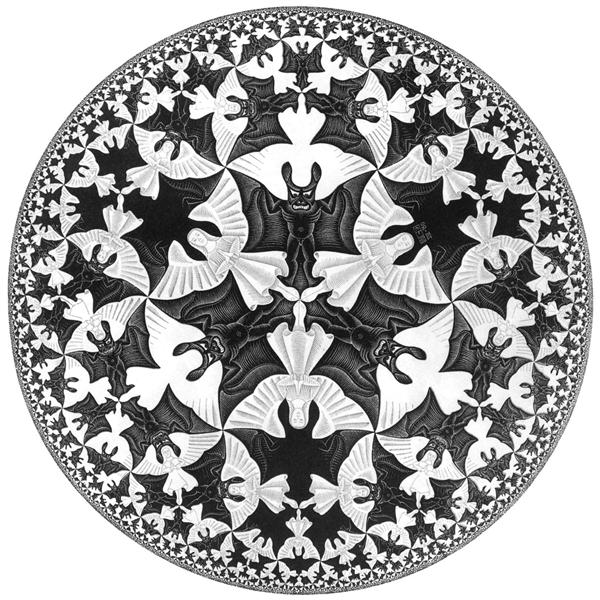
\includegraphics[width=0.6\textwidth]{a.jpg}
  \end{figure}
\end{frame}

\begin{frame}
  \frametitle{\(\CC \setminus (- \infty, 0]\)}
  \centering
  
\includegraphics[width=0.7\textwidth]{b.png} % replace with your filename
\end{frame}

\begin{frame}
  \frametitle{Desna polrvnina}
  \centering
  
\includegraphics[width=\textwidth]{c.png} % replace with your filename
\end{frame}

\begin{frame}
  \frametitle{Pas}
  \centering
  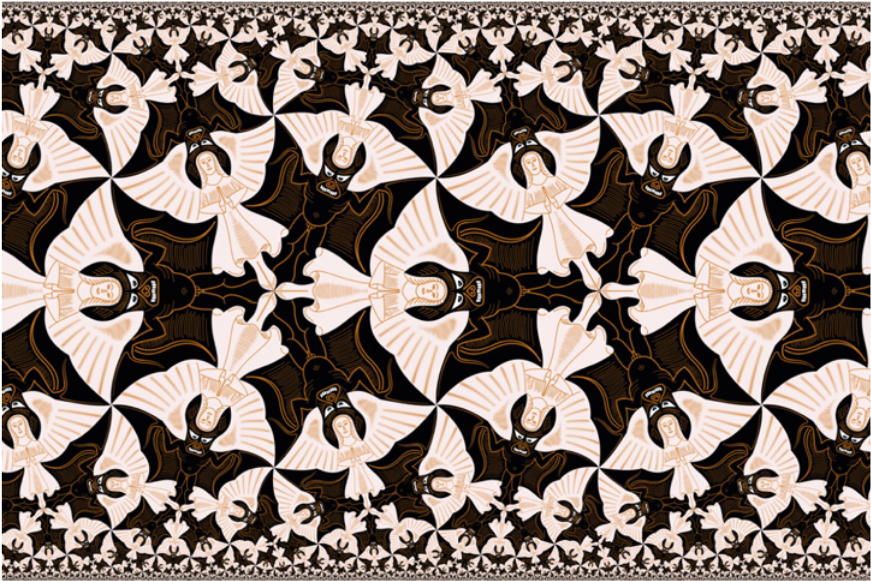
\includegraphics[width=\textwidth]{d.png} % replace with your filename
\end{frame}

\begin{frame}
  \frametitle{Delovanje eksponentne preslikave}
  \centering
  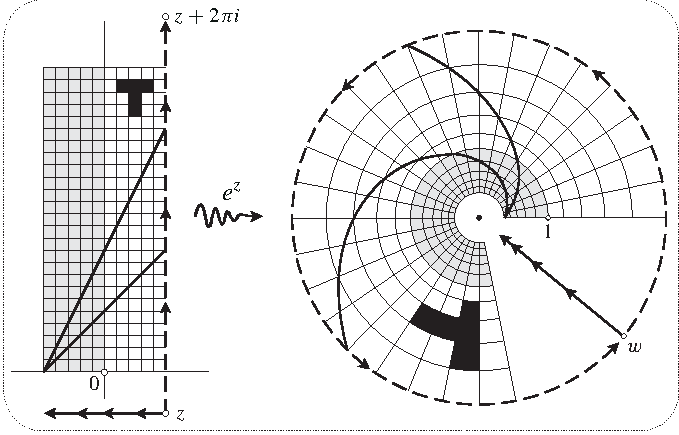
\includegraphics[width=\textwidth]{e.pdf} % replace with your filename
\end{frame}

\begin{frame}
  \frametitle{Občutljivost na začetne pogoje}

  \begin{block}{Dodatni izrek}
    Naj bo \(W \subset \CC\) odprta in neprazna. Potem za neskončno mnogo \(n \in \NN\) velja \(f^{n} (W) \cap (- \infty, 0] \neq \emptyset.\)
  \end{block}

  \begin{block}{Občutljivost na začetne pogoje}
    Naj bo \(X \subseteq \CC\) in \(d\) metrika na \(X\). Zvezna preslikava \(f \colon X \to X\) je \emph{občutljiva na začetne pogoje}, če obstaja tak \(\delta > 0\), da za vsako odprto množico \(U \subseteq X\) obstajata \(x, y \in U\), da velja \(d(f^n(x), f^n(y)) > \delta\) za nek \(n \in \NN\).
  \end{block}

  \begin{block}{Občutljivost v sferični metriki}
    Zvezna preslikava \(f \colon \CC \to \CC\) je \emph{občutljiva na začetne pogoje glede na sferično metriko}, če obstajata \(\delta > 0\) in \(R > 0\), tako da za vsako odprto in neprazno množico \(U \subset \CC\) obstajata \(z, w \in U\) ter \(n \geq 0\), da velja \(\vert f^n (z) \vert \leq R\) in \(\vert f^n (z) - f^n (w) \vert \geq \delta\).
  \end{block}

\end{frame}

\end{document}